
\section{Distributed optimization with ADMM}

\textbf{Goal}
Solve s.t. each term can be handled by its own processor.
\vspace{-2mm}
\begin{equation}
	\min_{x_1..,x_N, z \in \mathbb{R}^{n}}
	\sum_{i = 1}^{N} f_i(x_i)
	\quad\text{s.t.}\quad x_i=z
	\quad(f_i \text{ convex})
	\label{eq:sum_distributed}
\end{equation}

\begin{center}
	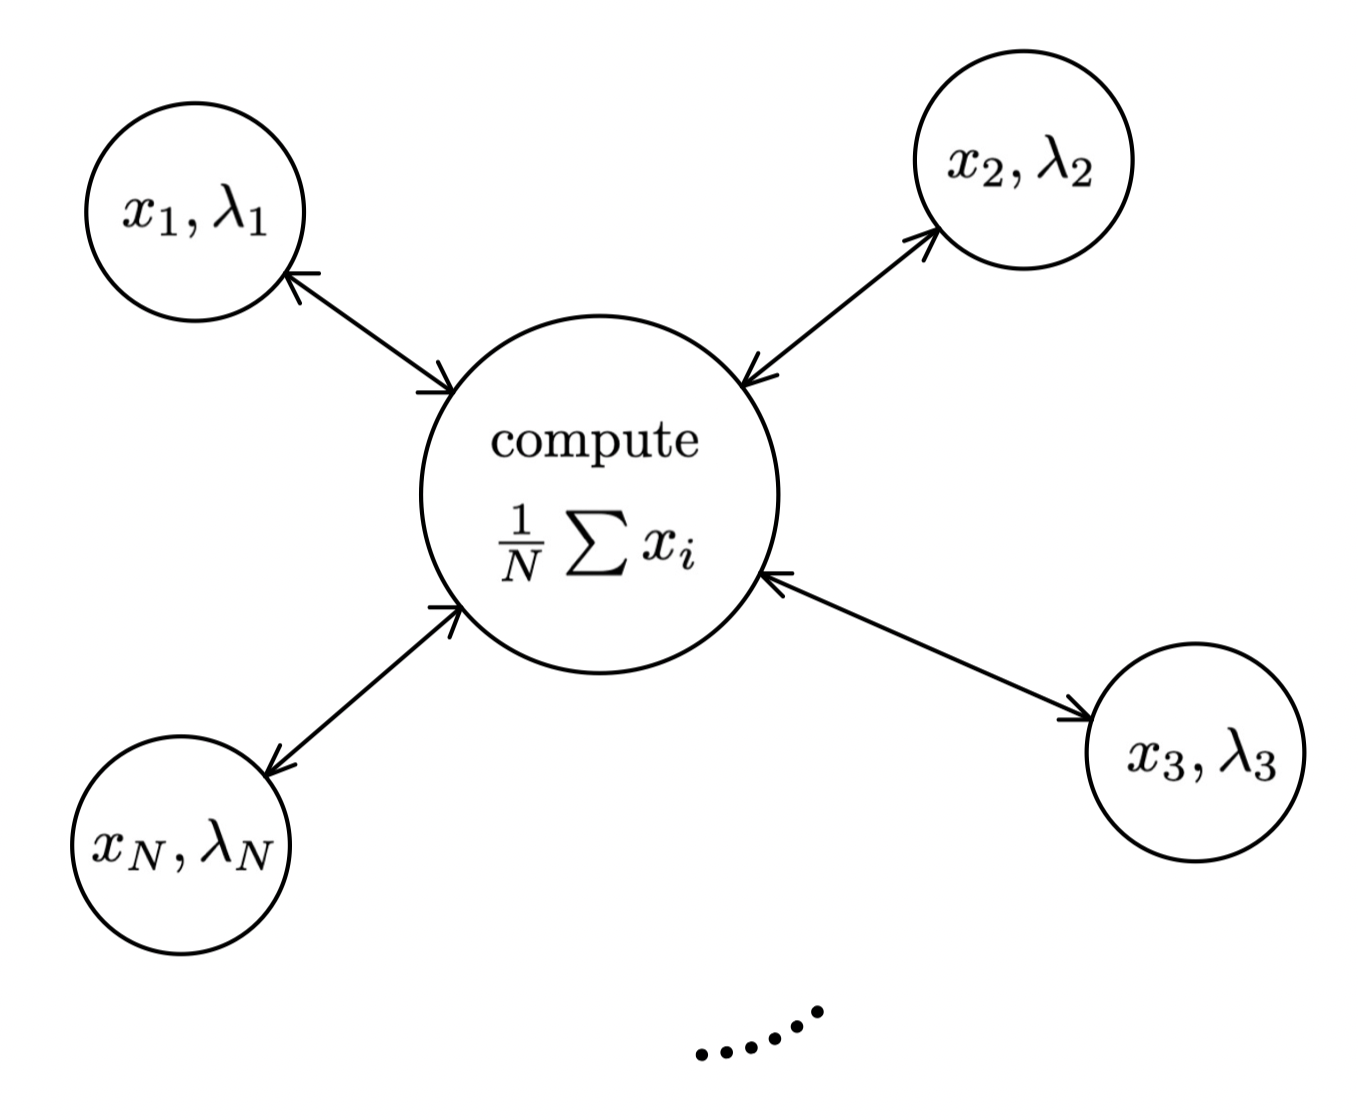
\includegraphics[width=0.92\columnwidth]{images/distributed.png}

	(Distributed ADMM)
\end{center}
\subsection{Global Consensus Problem}

Step 1: Augmented Lagrangian% $i\in[1,N]$
\vspace{-2mm}
to solve (\ref{eq:sum_distributed}) with ADMM.

$$\begin{aligned}
		\mathcal{L}_p(x_i,..,\lambda_i) & =
		\sum_{i=1}^{N}f_i(x_i)
		+\lambda_i\T(x_i-z)+\frac{\rho}{2}|x_i-z|^2
		\\
		                                & =\sum_{i=1}^{N}f_i(x_i)
		+\frac{\rho}{2}|x_i-z+\frac{1}{\rho}\lambda_i|^2-\frac{1}{2\rho}|\lambda_i|^2
	\end{aligned}$$

Step 2: Formulate ADMM
$$\begin{aligned}
		x_i^{k+1} & = \underset{x_i\in\mathbb{R}^{n}}{\operatorname{argmin}}
		f_i(x_i)+\frac{\rho}{2}|x_i-z^k+\frac{1}{\rho}\lambda_i^k|^2
		\\
		z^{k+1}   & = \underset{z\in\mathbb{R}^{n}}{\operatorname{argmin}}
		\frac{\rho}{2}\sum_{i=1}^{N}
		|x_i^{k+1}-z+\frac{1}{\rho}\lambda_i^k|^2
		\\&=\frac{1}{N}\sum_{i=1}^{N}
		(x_i^{k+1}+\frac{1}{\rho}\lambda_i^k)
		\\
		\lambda_i^{k+1}
		          & =\lambda_i^k+\rho(x_i^{k+1}-z^{k+1})
	\end{aligned}$$

FURTHER REFORMULATIONS...


\subsection{Sharing Problem}

\begin{equation}
	\min_{x_1,..,x_N \in \mathbb{R}^{n}}
	\sum_{i = 1}^{N} f_i(x_i)
	+g\left(\sum_{i = 1}^{N}x_i\right)
\end{equation}

$\rightarrow$ copy all the variables $x_i=z_i$

$\rightarrow$ formulate augmented Lagrangian

$\rightarrow$ state ADMM dynamics

\subsection{Optimization over Graphs}


$g=(V,E)$ undirected graph with vertices $V$ and edges $E$

$$\begin{aligned}
		\min_{x \in \mathbb{R}^{n}} \sum_{i\in V} f_i(x)
		\Rightarrow
		 & \min_{x_i\in|V|,z_i\in|E|} \sum_{i\in V}^{N} f_i(x_i)
		\\&\text{s.t. }x_i=z_{ij}, x_j=z_{ij}\quad \forall(i,j)\in E
	\end{aligned}$$

Step 1: Augmented Lagrangian

Step 2: Form the Algorithm

ALGORITHM
\begin{align*}
	x_i^{k+1}       & = \arg\min_{x_i \in \mathbb{R}^n} f_i(x_i) + \frac{d_i}{2} \left| x_i - \frac{1}{2} (x_i^k - \bar{x}_i^k) + \frac{1}{\rho} p_i^k \right|^2, & \text{(local update)}                  \\
	\bar{x}_i^{k+1} & = \frac{1}{d_i} \sum_{j \in \mathcal{N}_i} x_j^{k+1},                                                                                       & \text{(communication with neighbours)} \\
	p_i^{k+1}       & = p_i^k + \frac{\rho}{2} (x_i^{k+1} - \bar{x}_i^{k+1}),                                                                                     & \text{(local update)}
\end{align*}
